\documentclass[aspectratio=169]{beamer}

\graphicspath{{../reports/figures/}}

\usepackage{cmap}
\usepackage[T2A]{fontenc}
\usepackage[utf8]{inputenc}
\usepackage[english,russian]{babel}
\usepackage{tikz}
\usepackage{array}
\usepackage{multicol}
\usepackage{booktabs}
\usepackage{csquotes}
\usepackage{amssymb,amsfonts,amsmath}

\usecolortheme{beaver}
\usefonttheme[onlymath]{serif}  % математика тем же шрифтом, что в статье
\setbeamertemplate{navigation symbols}{}
\setbeamertemplate{footline}[page number]
\setbeamertemplate{blocks}[rounded=true,shadow=true]
\setbeamersize{text margin left=0.5cm,text margin right=0.5cm}
\setbeamerfont{author}{size=\normalsize}
\setbeamerfont{institute}{size=\normalsize}
\setbeamerfont{date}{size=\normalsize}

\title[Разреженная поверхность волатильности]{Восстановление и прогнозирование разреженной поверхности подразумеваемой волатильности с учётом истории и связей между контрактами}
\author{
    Имя Фамилия\\
    Научный руководитель: Имя Фамилия, к.ф.-м.н.\\
    Консультант: Имя Фамилия, к.ф.-м.н.
}
\institute{
    МГУ имени М.\,В.~Ломоносова
}
\date{2026}

\begin{document}

\begin{frame}
    \thispagestyle{empty}
    \maketitle
\end{frame}

\begin{frame}{Поверхность волатильности на разреженном рынке}
    Поверхность $\sigma(k, T)$ нужна для оценки опционов и рисков, но рынок видит её в немногих точках.
    \begin{block}{Цель}
        Выяснить, помогают ли история и связи между контрактами восстанавливать и прогнозировать поверхность лучше классических безарбитражных методов при малом числе текущих наблюдений.
    \end{block}
    \begin{block}{Проблема}
        SVI/SSVI и сплайны строят поверхность по текущей доске "--- при разреженности им не хватает данных.
    \end{block}
    \begin{block}{Подход}
        \begin{enumerate}[1)]
            \item Скрывать реальные наблюдения при контролируемой разреженности.
            \item Сравнивать методы текущей доски с методами, использующими историю.
            \item Оценивать точность вместе с арбитражем и режимами.
        \end{enumerate}
    \end{block}
\end{frame}

\begin{frame}{Идея на одном слайде}
    Расчётная кривая биржи плотная, но модельная; реальные наблюдения "--- сделки: их мало и они шумные. История плотных кривых доступна за много лет.
    \begin{figure}
        \centering
        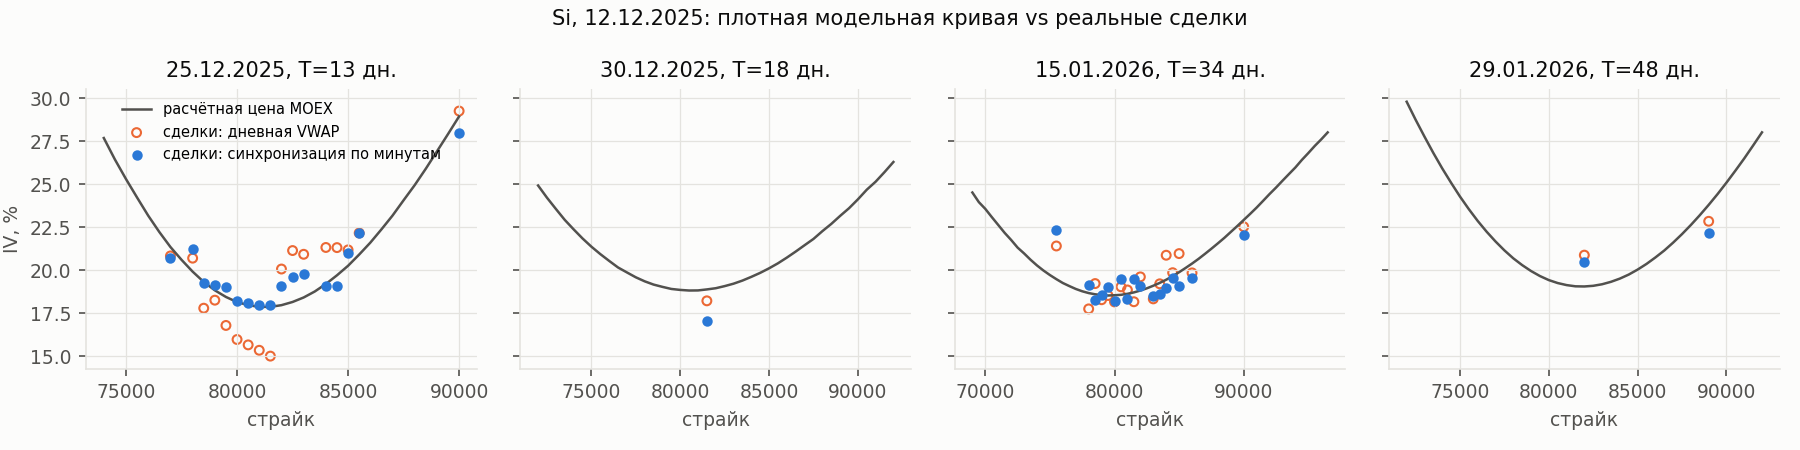
\includegraphics[width=\textwidth]{example_day_Si}
    \end{figure}
    \textbf{Вопрос:} сколько информации добавляет история к разреженной текущей доске?
\end{frame}

\begin{frame}{Постановка задачи}
    Доска дня $t$: наблюдения $\mathcal{O}_t = \{(k_i, T_i, \sigma_i)\}_{i=1}^{n_t}$, где $k = \ln(K/F)$; история $\mathcal{H}_{t-1} = (S_{t-1}, S_{t-2}, \dots)$ "--- предыдущие поверхности.
    \begin{block}{Восстановление}
        Видна часть доски $\mathcal{O}^{\mathrm{vis}}_t \subset \mathcal{O}_t$; требуется $\hat\sigma_t(k, T) = f\bigl(\mathcal{O}^{\mathrm{vis}}_t, \mathcal{H}_{t-1}\bigr)$, ошибка считается в скрытых точках $\mathcal{O}_t \setminus \mathcal{O}^{\mathrm{vis}}_t$.
    \end{block}
    \begin{block}{Прогноз}
        $\hat S_{t+h} = g(\mathcal{O}_{\le t})$, оценка только на хронологически будущих данных.
    \end{block}
    \begin{block}{Финансовая корректность}
        Выпуклость цены колла по страйку (бабочка) и неубывание $w(k, T) = \sigma^2 T$ по $T$ (календарь).
    \end{block}
\end{frame}

\begin{frame}{Данные MOEX: что есть в открытом доступе}
    \begin{columns}
    \begin{column}{0.5\textwidth}
        \textbf{Доступно}
        \begin{itemize}
            \item итоги дня по каждому опциону с 2001~г.: сделки, объём, открытый интерес, расчётная цена;
            \item минутные свечи опционов и фьючерсов "--- синхронизация IV сделок с базовым активом;
            \item текущие лучшие bid/ask с задержкой.
        \end{itemize}
    \end{column}
    \begin{column}{0.5\textwidth}
        \textbf{Недоступно бесплатно}
        \begin{itemize}
            \item исторические bid/ask и стаканы;
            \item готовые исторические кривые волатильности.
        \end{itemize}
        \medskip
        \textbf{Следствие:} целевые наблюдения "--- сделки; расчётная кривая биржи "--- плотная история и сильный ориентир, но не истина.
    \end{column}
    \end{columns}
\end{frame}

\begin{frame}{Разреженность реальна}
    \begin{figure}
        \centering
        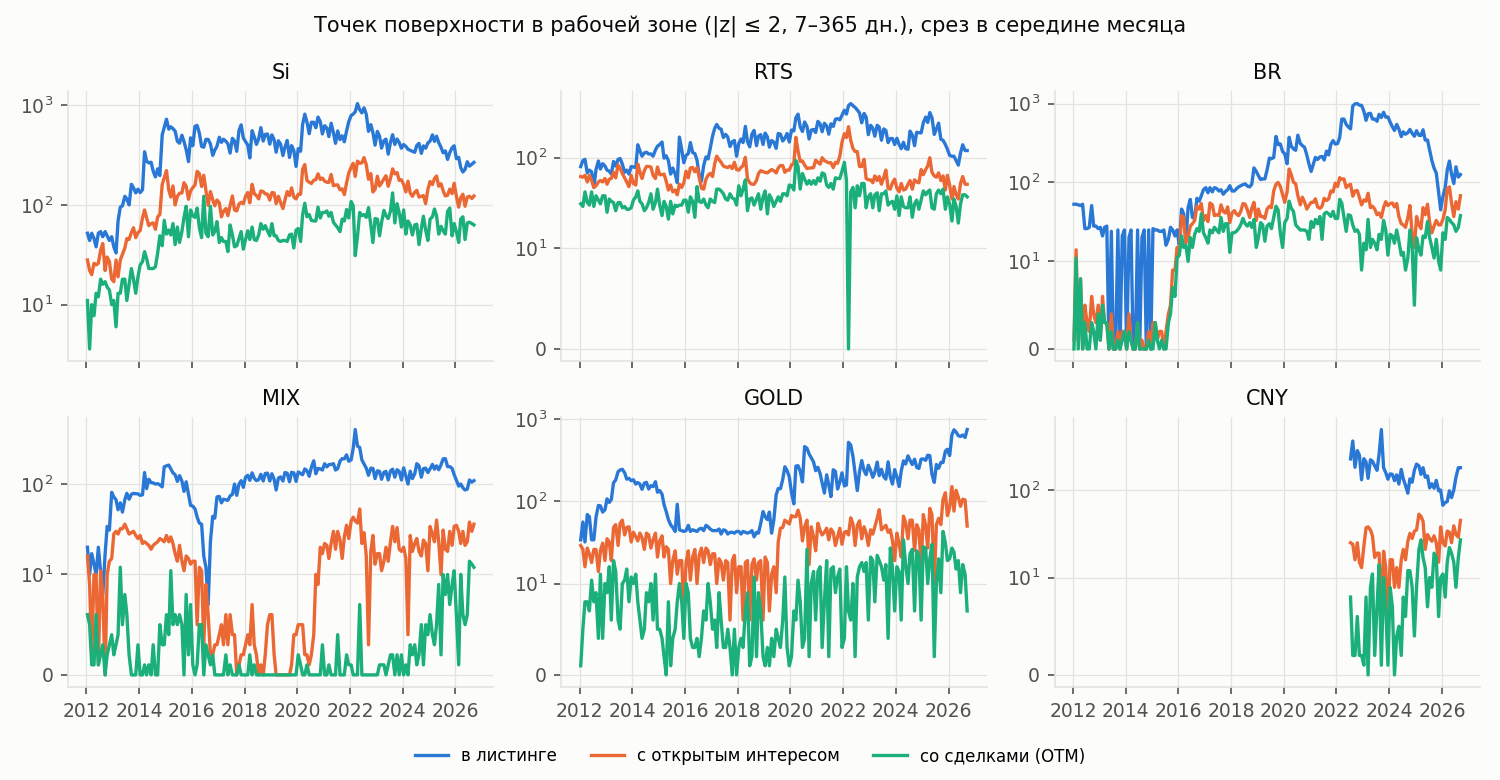
\includegraphics[width=0.85\textwidth]{density_monthly}
    \end{figure}
\end{frame}

\begin{frame}{Пилот: история против текущей доски}
    \begin{columns}
    \begin{column}{0.4\textwidth}
        Si, 254 дня, 21\,217 сделок: скрываем долю сделок дня и восстанавливаем их по остальным.
        \begin{itemize}
            \item только текущая доска: квадратичная улыбка, SVI;
            \item только история: вчерашняя кривая;
            \item история + текущая доска.
        \end{itemize}
    \end{column}
    \begin{column}{0.6\textwidth}
        \begin{figure}
            \centering
            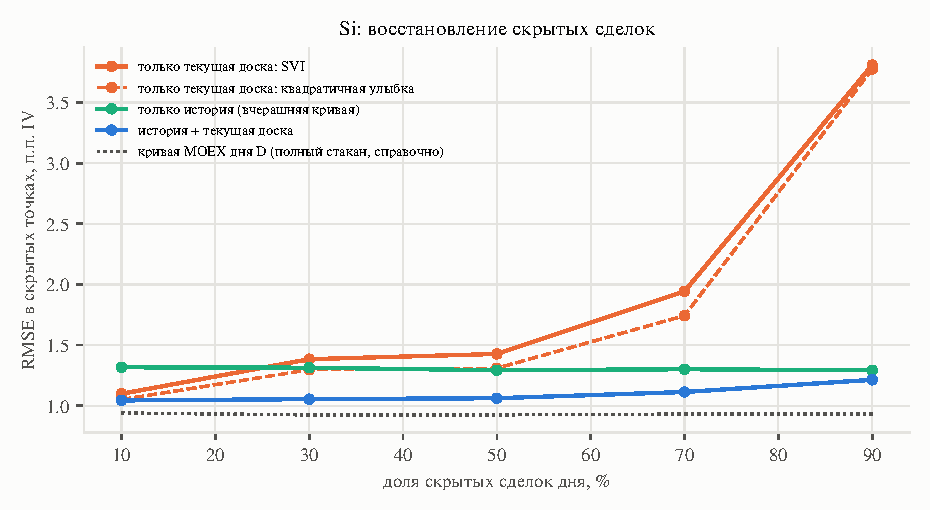
\includegraphics[width=\textwidth]{pilot_masking_Si}
        \end{figure}
    \end{column}
    \end{columns}
\end{frame}

\begin{frame}{Выводы и дальнейшие шаги}
    \begin{enumerate}[1)]
        \item Задача: восстановление и прогноз поверхности по разреженной доске MOEX; основной актив "--- Si, проверка "--- RTS.
        \item Реальные наблюдения "--- сделки: у Si около 20\,\% точек листинга в рабочей зоне; расчётная кривая биржи плотная, но модельная и несогласована по срокам.
        \item Пилот: при 10\,\% скрытых сделок история не помогает; при 50--90\,\% и на крыльях история + текущая доска заметно лучше методов только текущей доски.
        \item Наивный перенос поправок между сериями вредит "--- связи между контрактами нужно моделировать структурно.
        \item Далее: SSVI и безарбитражные сплайны, факторная динамика, модели со связями между сериями, контроль арбитража, прогноз на $t+h$.
    \end{enumerate}
\end{frame}

\end{document}
